\chapter{Concept}\label{Chap:Concept}

This chapter will explain what requirements were defined for the to be built system and how it will be designed and setup. For further reading the system will be called "Parametrised Augmented Reality Robot Human Interface" (\textit{PARRHI}).

\section{Goal, Requirements and Use Cases}
As described in section \ref{Section:PARRHIApproach} this thesis presents a possible approach to solve the previously described problems (see section \ref{Section:ProblemDescription}). It is the main target of this bachelor's thesis to remove the necessity of high software engineering skills to develop reasonably complex Augmented Reality Robot Human Interface applications, maintaining the quality of the outcome and even increasing the degree of resuability. This might result in lower development costs, lower struggle to gather software engineering talent and even in a shorter time to market.

To succeed in this goal, a specific set of requirements has to be defined and documented in a formal way. To gather these requirements the V-Model developed by the Federal Republic of Germany was used~\cite{vmodell}.

\subsection{User Requirements}
Before defining the User Requirements the system's end user has to be defined. The characteristics of the actual enduser of \textit{PARRHI} might be someone who:
\begin{itemize}
	\setlength\itemsep{-1em}
	\item Knows the basics of text editing software,
	\item has no qualifications in software engineering,
	\item wants to develop an Augmented Reality application for professionals that collaborate with industrial robots in a shared perimeter.
\end{itemize}

Having an idea of the end-user, the user-requirements can be defined. The user wants to:
\begin{itemize}
	\setlength\itemsep{-1em}
	\item Develop a AR-applications without software engineering skills
	\item Have the tools necessary to create medium complex applications for use cases such as tutorials, maintenance instructions or other teaching purposes
	\item Build upon other people's work or projects
	\item Launch the AR-application on a suitable device
	\item Possibly use the same system on different types and brands of robots
\end{itemize}

\subsection{System Requirements}\label{Section:SystemRequirements}
Deriving from the previous chapter the System should:
\begin{enumerate}
	\setlength\itemsep{-1em}
	\item have user input in a simple and intuitive format to allow for non-software engineers.
	\item have readable and intuitive feedback on every user input.
	\item achieve reusablity by having an input in non-binary text format that allows copy and paste reproduction.
	\item support building for hand held mobile devices and head mounted Augmented Reality glasses.
	\item allow bidirectional communication with the real and virtual world in different formats
	\item allow documentation of the application's workflow
	\item be as platform independent as possible
\end{enumerate}

\subsection{Possible Use-Case: Factory Maintenance}
This section depicts a possible use case example for the PARRHI system, especially how and why it could be used. One could imagine a huge auto mobile factory with hundreds of industrial robots assembling certain parts of a car. A factory like this, might want to repeatedly check on their robotic infrastructure to recognise problems and thus avoid any future downtime. The difficulties here are, that one generally does not want a robot to not be in operation due to the high costs of it but on the other hand non-collaborative robots are dangerous and can inflict damage on humans and other property, which means that the robot should be switched off or at least in a safety mode while humans are around. Thus, the operator should be quick and precise in their task without letting down their security safe guard.

Despite being expensive, finding employees that have the necessary skills is not an easy task. Hence it would be interesting to teach new personnel how to succeed in these very specific cases. An Augmented Reality application might be the right approach for cases like these. For every specific maintenance task an employee knowledgable enough could develop AR applications, which lead a small army of less-skilled workers through their tasks step by step without ever compromising their safety.

Developing such a high number of AR-applications is not really plausible with current frameworks. Despite the knowledgable employee probably not having enough programming skill, it might simply be too expensive, slow and too hard to adapt to new changes. A system like PARRHI would allow the skilled employee to write these applications themself without the need of software engineers. Since many tasks might be similar to one another, the employee could re-use most of the applications program over and over again - further increasing development speed. PARRHI applications will be able to involve the Real World's data in their workflow, which allows the application to know where the robot currently is located and command the maintenance worker to move away. Having the possibility to also influence the Real World, the application could hinder the robot from moving, while the employee is in a certain danger area. All that, while showing instruction steps in Augmented Reality to easily understand and complete the task quickly.

In essence, using systems like PARRHI might reduce the development costs of AR-applications substantially, which could open a wide set of use cases, that were untouched before due to the high costs. This might allow for a much better economically usage and a much wider set of real world applications for Augmented Reality apps. 

\clearpage
\section{PARRHI Concept}

The following chapter will now explain the concept of the PARRHI system and show one possible approach to reach the previously mentioned requirements.

\begin{figure}[h]
	\centering
	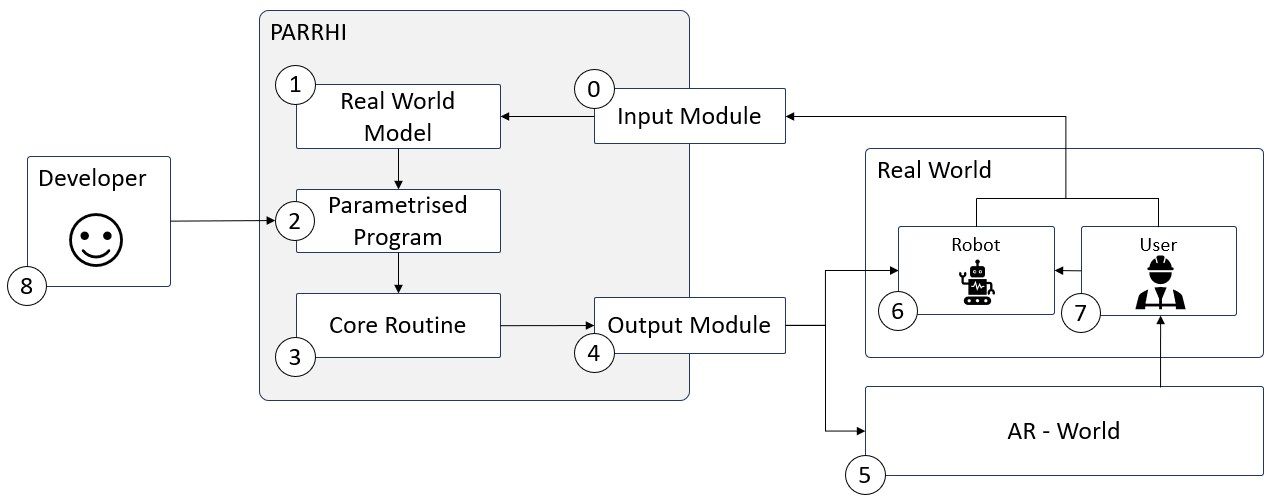
\includegraphics[width=1\textwidth]{Figures/PARRHIConcept03.jpg}
	\caption{PARRHI general concept}
	\label{Fig:PARRHIConcept}
\end{figure}

Fig. \ref{Fig:PARRHIConcept} depicts PARRHI's concept, which consists of three main parts. The left hand side shows the developer and his workflow. The grey box in the middle is the PARRHI system itself. Lastly, the right side visualises the environment that surrounds the PARRHI system in both virtual and real space. I will now go into detail and systematically explain each component from (0) to (8), before describing the information flow between them.

\begin{enumerate}
	\addtocounter{enumi}{-1}
	\setlength\itemsep{-1em}
	\item Input Module: The Input Module (0) is responsible for collecting data needed for the PARRHI system from the real world. In this specific case, it  receives the robot's (6) joint angles and the user's (7) position.
	\item Real World Model: In order to utilize data from the Input Module (0) it has to be processed. The Real World Model (1) has a deeper understanding about the real world and helps to extract useful information from the data inflow. In this specific case, its outputs are the robot's (6) joint positions and the user's (7) location represented as parameters that are available for the Parametrised Program (2).
	\item Parametrised Program: This is a document that defines the AR application's behaviour and workflow. Its syntax is parametrised, meaning, that it makes use of placeholders (parameters) whose actual value is managed by PARRHI itself at runtime. There are two types of parameters. First, there are the ones that are provided by the Real World Model (1) (for example the discussed robot's (6) joint positions and the user's (7) location) and secondly any object defined in the Parametrised Program itself (2) can act as a parameter for other objects in the program. These objects can be 3D AR-Hologram definitions, logical instructions or a variety of events and actions. For a more thorough explanation of the Parametrised Program see section \ref{Chap:ParametrisedProgram}.
	\item Core Routine: The Core Routine (3) is an interpreter for the Parametrised Program (2), and acts on its instructions. It generates the output of the application which can either be commands to the robot (6) and thus real world, or instructions for the AR-World (5).
	\item Output Module: This component manages the outgoing communication with PARRHI's environment. 
	\item AR-World: The Augmented Reality World is the space, where a part of PARRHI's output is displayed. It can display holograms like spheres and cylinders, but also written text for instructions. The AR-World (5) augments the Real World and is thereby seen by the User (7) through an AR Device.
	\item Robot: It is a Real World object that can be controlled by the User (7) themselves, or by the PARRHI system.
	\item User: This is the person that would use the finished application to fulfil their task, which could for example be to do some work following instructions, or to simply learn different aspects about the robot/working environment.
	\item Developer: This person develops the application's workflow and behaviour. Their output is the Parametrised Program (2) as a text-based document, which is then fed into the PARRHI system after being validated. 
\end{enumerate}

It should now be clearer what each component is responsible for. After having laid down the fundamentals, the following paragraph will track the information flow between the components. The order will be a bit different here, since it will be built up in a chronological way. Hence, I will first start with the Developer (8) crafting the Parametrised Document and then continue with the standard runtime cycle of the PARRHI system.

After having defined what the AR-HR-Interface application should achieve, the Developer (8) crafts the Parametrised Program (2). The text-based hierarchically built document will be validated first, before it is granted access into the PARRHI system. If the validation fails, the Developer (8) receives error messages accordingly an can reiterate over his document until it validates successfully.

The runtime loop starts with the Input Module (0). As described, it not only collects the robot's (6) joint angles, location and gripper-state but also the User's (7) position. This input data is then fed into the Real World Model (1), which uses its Real World understanding to extract/calculate useful information. In this specific case, it applies forward kinematics onto the robot's (6) joint angles to calculate their 3D position and transforms the User's (7) location coordinates into PARRHI's internal coordinate system. After transforming the input data into a usable format, the Parametrised Program (2) comes into play. The Developer (8) wrote this document in a parametrised way using placeholders. The latter are now filled with information by the PARRHI system. For example, the Parametrised Program (2) could use the robot's tool centre point (TCP) for a definition of some AR-holograms, without knowing where exactly the TCP is during development. At runtime, PARRHI inserts this information into the parameters. 

The Core Routine (3) then interprets the now-filled-in Program (2). It first updates its internal state with the new parameters, before updating all AR-Holograms. At last it evaluates all events, and triggers their actions if needed. These actions might be commands for the AR-World (5) (for example to show or hide holograms, or to change UI text) or commands for the Real World Robot (6) (e.g. to move or stop the robot). These commands are passed into the Output Module (4), which is responsible for actually executing them. It has the required tools to communicate with the robot and with the AR - World (5). 

At this point, the User (7) sees two things. On one hand they see the Real World in front of them. There is the Robot (6) and a surrounding environment. The Robot (6) might be instructed to do something by the Output Module (4) already. Superimposed onto the Real World they see the Augmented Reality World (5), which contains all visual information, that the Output Module (4) constructed. There could be cylindrical translucent holograms marking a danger zone around the robot's (6) axes. Now, the AR-World's (5) content influences the User (7) to do certain things. He could be instructed by holograms to move into a safe-zone. At the same time, the User (7) might control the Robot (6). At this point it is to mention, that the Output Module (4) enjoys priority over the User's (7) input when commanding the Robot (6).

As Fig.~\ref{Fig:PARRHIConcept} depicts, the Input Module (0) then finally closes the feedback loop by receiving fresh data from the Real World. The information flow that was followed in the paragraphs above changed the environment either by direct commands or indirectly by commanding the User (7) via the AR World (5). These changes will now be reflected in the input data and are thus available for the next cycle. The presented loop repeats itself, where every iteration only takes a fraction of a second, until the PARRHI system is terminated for some reason. 

The preceding paragraphs should give a relative detailed overview about the concept behind PARRHI. The following chapters will now explain each part in an even higher degree of detail, with the goal being, that almost no questions about the concept stay unanswered. The order will be similar to the explanation of the information flow in the PARRHI concept, meaning, that the Input Module (0) and the Real World Model (1) will be explained first, followed by a very thorough explanation of the Parametrised Program (2) with all its objects and definitions. In the end the Core Routine (3) and the Output Module (4) with the Real and AR-World (5) will finish off the concept chapter.


% As discussed, parametrising workflows grants a multitude of benefits (see section~\ref{Section:ParametricDesignIntoduction}). Disclosing pre-processed information to the application program via parameters, mitigates the development effort substantially by simplifying the developer's code-base, complexity and workload.  

% To offer these parameters in a meaningful format, \textit{PARRHI} needs a decent model about its surroundings (see (1) in Fig. \ref{Fig:PARRHIConcept}). The model then allows to extract helpful information from complicated environments. In \textit{PARRHI's} case, this model includes the robot's forward kinematics. The developer may now use this implicitly known and automatically retrieved information in the application program (2) without necessarily understanding the source's background and mathematics. \textit{PARRHI} will retrieve, calculate and update these parameters at runtime, "filling in the gaps".

% The parametrised program (2) is an exchangeable document, provided by the application developer. Here, the application's workflow and output is defined using the afore mentioned placeholders and an additional set of tools for logic operations, also utilizing parameters. The Core Routine (3) then interprets the parametrised program and generates the output, which may act on both the virtual and real world via the Output Module (4). The real world is manipulated by (e.g.) commanding the robot in some way, whereas the virtual space may be changed by displaying UI, holograms or other augmentations. The Input Module (0) finally closes the feedback loop by sensing the environment. Information from the real world (user's position) and the robot's joint-position are fed into the Real World Model (1) before being combined with data about the virtual space (position and state of holograms), thereby contributing to the implicit knowledge about the environment.

% Actions in both the real and virtual space may influence the other in some way. A hologram hinting the user to move their location originated in the virtual space but directly influenced the user - a real world object. Also the other way round, if a hologram is parametrised to cover the robot, the machine's movement also influences the virtual space because the parameters are updated constantly.



% The following chapters will describe the underlying system parts ((1) - (5)) in more detail, including some examples how something might be used. 


\subsection{Preparation of Parameters}
One main strength of the \textit{PARRHI} concept is its disclosure of its knowledge of the outside world to its inner components via parameters. Two steps are necessary to do exactly that. First, an Input Module (0) has to automatically retrieve real world information. Since the latter quite hard to comprehend for computer programs, some model knowledge (1) should be implemented to process the input data by reducing complexity. Generally, models are a more abstract version of the object it is supposed to describe. Next to being easier to understand, one benefit is, that one can often explain models in a mathematical way, which is of course perfect for computer programs. 

The complexity of collecting Real World data strongly depends on the use case. I decided to limit my scope to the collection of three things, since it is not the main focus of this thesis. Firstly, gathering the robot's location is a key aspect. For Augmented Reality applications, it is utterly important for the AR device to know its six dimensional orientation (position and rotation). Otherwise superimposed holograms would not make any sense to the viewer, since they appear misplaced. The centre of origin for \textit{PARRHI} applications should thereby always be the robot's base. 

Then of course the robot's joint positions are needed for the application program to offer the possibility to fully integrate the robot in the application's workflow. Since most robots do not offer their individual joint positions in 3D vectors but only their joint angles, a corresponding robot model is needed to calculate each joint's position from their joint angles. This is called forward kinematics, an old problem in robotics with known mathematical tools and ways to solve it. In principle, one can calculate a robot's tool point via every joint angle and some knowledge about the robot's configuration. The latter is specified by the types of joints (degrees of freedom (DOF)) and the distance between consecutive joints. A mathematical model then outputs each joint's three dimensional location, which is offered to the Application Program (2) via parameters. To get an example of how the joint's position might be used in a parametrised way see section~\ref{Section:Points}.

\clearpage
\subsection{Parametrised Program}
\label{Chap:ParametrisedProgram}
The Parametrised Program is the document, which the Developer ((8) in Fig. \ref{Fig:PARRHIConcept}) of the \textit{PARRHI} system crafts. It contains parametrised, hierarchically structured data, that defines the behaviour, feel and look of the final AR-HR-application. All instructions and definitions can make use of the previously explained parameters offered and maintained by \textit{PARRHI}. Since this is the actual document that a developer writes, its syntax and structure has to be as simple as possible to fulfil the requirements from section~\ref{Section:SystemRequirements} without limiting the developer's creativity. To achieve this, a rather natural way of describing the wanted behaviour was chosen. 

The following chapters explain the set of tools that are available to the developer, how they work and interconnect. Table~\ref{Table:InputDataStructure} displays the top level structure and its main parts, where Variables, Points and Holograms define assets that Events can work with. Each section will describe what exactly is parametrised in their definition and how they can be used as parameters to define other program parts.

\begin{table}[ht]
	\caption{\textit{Input Data} structure}
	\label{Table:InputDataStructure}
	\centering
	\begin{tabular}{lcl}
		\toprule
		Name & Section		& Explanation	\\		
		\midrule
		Variables & \ref{Section:Variables}		& Integer variables in a traditional sense \\
		Points& \ref{Section:Points}		& \parbox[t]{10cm}{Different kinds of 3D Point definitions\\(fix, relative to the robot, relative to the user)} 	 \\
		Holograms& \ref{Section:Holograms} & Holograms can be mounted onto points and have a set of properties\\
		Events& \ref{Section:Events} & Events have certain triggers and carry Actions as a payload \\
		\bottomrule
	\end{tabular}
\end{table}

\subsubsection{Variables}\label{Section:Variables}
Variables are storage locations for numbers and have a symbolic name. They can be used to create different steps in one's application. When using Variables as parameters, they can be the source of an event's trigger or the target of an event's action (see section~\ref{Section:Events}) and thus take part in the application's logic. With the help of Variables an application could keep track of something by counting events, or also implement state machines that jump between modes. Variables are internal knowledge, meaning, that they are managed by the \textit{PARRHI} system and are not imported/external information.

\subsubsection{Points}\label{Section:Points}
Points are probably the best example of parametrised information in the \textit{PARRHI} system. At runtime the data from the Real World Model (see (1) in fig.~\ref{Fig:PARRHIConcept}) is directly fed into the definition of all points that use the according parameters. Thus, the system updates these objects repeatedly with Real World information, that was fed through the Real World Model. Although points are defined using parameters in some way, points themselves are parameters to other objects in the Parametrised Program.
 
They essentially are a three dimensional vectors ($X$, $Y$, $Z$), with their coordinates being parameters. Depending on the type of Point, the parameters are set differently. There are three types of point definitions, with the difference between them being, what values are inserted into the $X$, $Y$ and $Z$ parameters.
\begin{enumerate}
	\setlength\itemsep{-1em}
	\item Fix-Point
	\item Robot-Point
	\item Camera-Point
\end{enumerate}

The \textbf{Fix-Point} has static coordinates and thus fixed values are used to define their coordinate parameters (see figure \ref{InputData:PointFix}). It could be used to setup holograms that visualize certain spacial environmental constraints or for different steps in a \textit{PARRHI} AR-HR-Interface application.

\textbf{Robot-Points} are defined by two indexes of the robot's joints and one scalar value that linearly interpolates between them (see figure~\ref{InputData:PointRobot}). The application's developer does not have to understand the robot's kinematics and simply uses the joint-indexes as parameters. At runtime, the \textit{PARRHI} system retrieves the robot's joint position, uses the Real World Model to calculate each joint's position and then feeds this data into the Robot-Points. The final point's position is calculated as follows (with s being the scalar value and $J_n$ the position vector of Joint $n$ which is an output of the Real World Model):
\begin{equation}
\boldsymbol{P} = \boldsymbol{J_1} + (\boldsymbol{J_2}-\boldsymbol{J_1}) * s
\end{equation}

\textbf{Camera-Points} are a way to involve the user's position in the application. Similarly to the Robot-Points, the \textit{PARRHI} system retrieves the cameras coordinates via the Input Module, feeds it through the Real World Model to map it onto the internal coordinate systems and finally periodically updates the Camera-Points with the new location data of the head mounted AR-Device.


\begin{figure}
	\begin{minipage}{0.45\textwidth}
		\centering
		

\tdplotsetmaincoords{60}{120} 
\begin{tikzpicture} [scale=0.01, tdplot_main_coords, axis/.style={->, black, thick}, 
vector/.style={-stealth,black,thick}, 
vector guide/.style={dashed,gray,thin}]

%standard tikz coordinate definition using x, y, z coords
\coordinate (O) at (0,0,0);

%tikz-3dplot coordinate definition using x, y, z coords

\pgfmathsetmacro{\ax}{100}
\pgfmathsetmacro{\ay}{100}
\pgfmathsetmacro{\az}{200}
\pgfmathsetmacro{\axSize}{200}

\coordinate (P) at (\ax,\ay,\az);

%draw axes
\draw[axis] (0,0,0) -- (\axSize,0,0) node[anchor=north east]{$x$};
\draw[axis] (0,0,0) -- (0,\axSize,0) node[anchor=north west]{$y$};
\draw[axis] (0,0,0) -- (0,0,\axSize) node[anchor=south]{$z$};

%draw a vector from O to P
\draw[vector] (O) -- (P);

%draw guide lines to components
\draw[vector guide]         (O) -- (\ax,\ay,0);
\draw[vector guide] (\ax,\ay,0) -- (P);
\draw[vector guide]         (P) -- (0,0,\az);
\draw[vector guide] (\ax,\ay,0) -- (0,\ay,0);
\draw[vector guide] (\ax,\ay,0) -- (0,\ay,0);
\draw[vector guide] (\ax,\ay,0) -- (\ax,0,0);
\node[tdplot_main_coords,anchor=north]
at (\ax+100,0,-60){(\ax, 0, 0)};
\node[tdplot_main_coords,anchor=west]
at (0,\ay,50){(0, \ay, 0)};
\node[tdplot_main_coords,anchor=south]
at (0,0,\az+50){(0, 0, \az)};
\end{tikzpicture}
		\caption{Fix-Point example}
		\label{InputData:PointFix}
	\end{minipage}\hfill
	\begin{minipage}{0.45\textwidth}
		\centering
		
\tdplotsetmaincoords{60}{120} 
\begin{tikzpicture}  [scale=0.03, tdplot_main_coords, axis/.style={->, black, thin}, 
vector/.style={-stealth,green,very thick}, 
robot/.style={green, very thick},
vector guide/.style={dashed,gray,thin}]

%standard tikz coordinate definition using x, y, z coords
\coordinate (O) at (0,0,0);

%tikz-3dplot coordinate definition using x, y, z coords


\pgfmathsetmacro{\axSize}{100}
\pgfmathsetmacro{\jointRadius}{50}

%Robot Points in cm (mm too large dimensions for library)
\coordinate (P0) at (0,0,0);
\coordinate (P1) at (5,0,33);
\coordinate (P2) at (5, 0, 77);
\coordinate (P3) at (15, 0, 100.5);
\coordinate (P4) at (47, 0, 100.5);
\coordinate (P5) at (55, 0, 100.5);
\coordinate (P6) at (63, 0, 100.5);
\coordinate (Point) at (5, 0 , 60);


%draw coordinate system axes
\draw[axis] (0,0,0) -- (\axSize,0,0) node[anchor=north east]{$x$};
\draw[axis] (0,0,0) -- (0,\axSize,0) node[anchor=north west]{$y$};
\draw[axis] (0,0,0) -- (0,0,\axSize) node[anchor=south]{$z$};

%draw the robot's joints and axes
\draw[robot] (P0) -- (P1); \fill[fill=gray] (P0) circle (\jointRadius pt);
\draw[robot] (P1) -- (P2); \fill[fill=gray] (P1) circle (\jointRadius pt);
\draw[robot] (P2) -- (P3); \fill[fill=gray] (P2) circle (\jointRadius pt);
\draw[robot] (P3) -- (P4); \fill[fill=gray] (P3) circle (\jointRadius pt);
\draw[robot] (P4) -- (P5); \fill[fill=gray] (P4) circle (\jointRadius pt);
\draw[robot] (P5) -- (P6); \fill[fill=gray] (P5) circle (\jointRadius pt);

%Draw PointRowot
\fill[fill=black] (Point) circle (\jointRadius pt);

%draw the 
\node[tdplot_main_coords,anchor=east]
at (P1){(Joint 1)};
\node[tdplot_main_coords,anchor=west]
at (P2){(Joint 2)};
\node[tdplot_main_coords,anchor=west]
at (Point){(Point scalar = 0.6)};




\end{tikzpicture}
		\caption{Robot-Point example}
		\label{InputData:PointRobot}
	\end{minipage}
\end{figure}


\subsubsection{Holograms}\label{Section:Holograms}
One of the main output channels of \textit{PARRHI} is the Augmented Reality World. The AR World can be filled with numerous objects (generally called holograms). In the Parametrised Program these Holograms are defined using parameters. In this case, Points are used to define the Hologram's location and orientation. Since Points are parametrised themselves, and are thus updated by the data from the Real World model, holograms are indirectly also strongly dependant of that feedback loop.

Holograms in the PARRHI system have a number of attributes. Holograms can be active (respectively also inactive), have a render-mode, a geometric definition and of course a location. The location is defined by a certain number of points - depending on the hologram's geometry. Currently the \textit{PARRHI} supports two types of holograms. There are spheres and cylinders, respectively taking one or two points and a radius as input parameters to define its size and position.

A Sphere's centre is always set to the point it was defined with, whereas a cylinder always connects the two points of its definition. All described types of points in section~\ref{Section:Points} can be used as input parameters for the location. With a given radius and point the three dimensional figure is well defined.

Holograms have an attribute called \textit{renderMode}, which if set to "transparent", renders the hologram in a half transparent way, allowing holograms to be used for boundary or zone visualizations. Furthermore the visibility of holograms can be changed by setting the \textit{active} parameter, which is done by actions as described in section~\ref{Section:Events}.

\subsubsection{Events}\label{Section:Events}
All previous elements (variables, points and holograms) exist to define the scene and to set up assets that can be utilized by events, which now actually describe the application's workflow. To do so, there are two subtypes in this category. There are event-triggers and event-actions (or short \textit{triggers} and \textit{actions}). Triggers have a boolean expression, which is checked periodically. As soon as the boolean expression evaluates to \textit{true}, the attached actions will be executed and the trigger will be disabled, avoiding multiple executions. One could say that if triggers the \textit{PARRHI's} sensors, actions are its tools to act on the augmentation. 

Triggers can be enabled and disabled, either from the beginning on, or toggled by an action. Every trigger has at least one action as a payload. To reach a reasonably capability numerous different but easy to understand triggers are available for the application's developer. In table~\ref{Table:Triggers} is a complete list of all defined triggers. \textit{(Note, that the enabled/disabled flag and actions are omitted in this table)}

 
 \begin{table}
 	\caption{Event Triggers}
 	\label{Table:Triggers}
 	\centering
 	\begin{tabular}{lll}
 		\toprule
 		Name & Input Parameter		& Trigger expression	\\		
 		\midrule
 		Distance trigger & Two Points $\boldsymbol{P_1}, \boldsymbol{P_2}$, distance $d$		&  $|\boldsymbol{P_2}-\boldsymbol{P_1}| \le d$ \\
		Variable trigger & Variable $v$, trigger value $v_{\text{tr}}$ 		& $v = v_{\text{tr}}$	 \\
		Time trigger & trigger time $t_{\text{tr}}$, time since enabling $t_{\text{enabled}}$ & $t_{\text{tr}} \geq t_{\text{enabled}}$\\
		\bottomrule
	\end{tabular}
\end{table}

\textbf{Distance trigger} can be used for two main purposes. First the application can use the robot's movement as an input using a \textit{Robot-Point}. An action could be triggered as soon as the user jogged the robot's TCP into wished position by using a \textit{Fix-Point} an waiting for them to come close to each other or to monitor the robot's joint position in Joint-Space by using two \textit{Robot-Points} as input parameters. Second the user's movement can be monitored by utilizing a \textit{Camera-Point} as an input. The application can thus ask the user to move to a specific location.

With \textbf{Variable triggers} the application is able to use defined variables as triggers. One could implement a counter for certain events, and trigger an action when a threshold value is reached. It can also be used for workflows that need states or steps. Finally the \textbf{Time trigger} allows the application to involve timers. The user could be given a maximum time for a task or holograms can be hidden after a few seconds.

Whenever a trigger's boolean expression evaluates to true, its actions are invoked and the trigger gets disabled. Since actions are the only way \textit{PARRHI} can influence the augmentation, there are numerous different types of actions - each serving a general purpose to fulfil the defined requirements (see section~\ref{Section:SystemRequirements}).

As with triggers, actions have a set of input parameters they need to fulfil their task. As with all other input data objects discussed so far, actions have a unique ID. The table~\ref{Table:Actions} gives a quick overview about all actions that \textit{PARRHI} currently supports.

\begin{table}
	\caption{Event Actions}
	\label{Table:Actions}
	\centering
	\begin{tabular}{lll}
		\toprule
		Action Name & Input Parameter		& Explanation	\\		
		\midrule
		Increment Counter  	& Variable $v$					& Increments the value of $v$ by 1 \\
		Set Hologram State 	& Hologram-IDs, State to set	& Enables/disables all specified holograms \\
		Set Trigger State  	& Trigger-IDs, State to set    	& Enables/disables all specified triggers \\
		Change UI Text	  	& Text to set					& Sets the UI Text\\
		Move Robot			& Point $P$						& Moves the robot to $P$ \\
		Set robot-hand State & State to set (open/close)		& Opens or closes the robot's gripper \\
		\bottomrule
	\end{tabular}
\end{table}

\textbf{Increment-counter actions} increment their integer variable by 1. If a developer wanted to count the number of times a user jogged the robot into a specific region, an Increment-counter action could be used as a payload of a Distance trigger. After a threshold value is reached, a Variable trigger could change the UI text and display a hint.

The \textbf{Set-Hologram-State action} enables hiding and showing holograms at runtime. If a hologram represents a region for a tutorial step, it can be hidden after the user's task is completed. The new scene can then be setup by displaying new holograms that guide the user's way. Another possible use would be, to display a warning boundary, if the user moves into a forbidden zone. This can be achieved by combining Distance trigger and Set-Hologram-State actions.

When using \textit{PARRHI} the user is presented a GUI that shows text and some other few options. The \textbf{Change-UI-Text action} allows to change this displayed text. There are numerous obvious use-cases where this is useful. Whenever it is of value to inform the user about something that cannot be achieved by holograms, this is a simple way to do so.

To create meaningful and longer applications, enabling and disabling triggers is an essential tool. This is what the \textbf{Set-Trigger-State action} is for. Triggers can only invoke their payload actions, if they are active. Triggers can either be defined as disabled from the beginning on, or get disabled by triggering as described above. The Set-Trigger-State action has the ability to (re)activate disabled triggers. There is a speciality in the case of \textit{Time triggers}. Their inner timer starts ticking, whenever they get enabled. This allows for timers to be used in the middle of applications, relative to other events.

\subsection{Core Routine}

\subsection{I/O Modules}
























